

\chapter{Dataset: Max Planck Institute Grand Ensemble CMIP6}
\label{ch:dataset}

\section{Overview}

The dataset chosen for this project is the \ac{mpige6}, presented by \cite{olonscheck_new_2023}. 
It is a single-model initial-condition large ensemble (in short: SMILE) consisting of multiple, coupled models: ECHAM6\footnote{\label{fn:modelname}Labels of the different models} for the atmosphere directly coupled to JSBACH\cref{fn:modelname} for land and MPIOM\cref{fn:modelname} for sea and sea-ice. 
The models are coupled once a day, which means that the simulation results of the different models serve as input for the other models.
As an ensemble simulation, it consists of multiple members, which are different variants of the simulation with the same forcings (such as \acp{ghg}) but different initial conditions. 
To generate the initial conditions, the historical simulations are split from 1000-year quasi-stationary preindustrial control simulation circa 25 years apart for each member, and the results of them in the year 2015 serve as the initial state for each corresponding member in the future scenarios. \cite{olonscheck_new_2023}
% This means that a single model was run with different initial conditions but the same external forcings (e.g., greenhous gasses) mutiple times. 
% Every seperate intial condition is a member of the simulation, and all members together are the whole ensemble. \cite{olonscheck_new_2023}

 

Differences from its predecessor MPI GE \cite{maher_max_2019} (which was used in the work of \citeauthor{vietinghoffdiss} \cite{vietinghoffdiss}) include improved time resolution (from monthly means up to 3 or 6 hour intervals) and the updated CMIP6 forcings and future scenarios (see Section~\ref{sec:scenariomip}). 
Since \ac{mpige6} follows the CMIP6 protocol (see Section~\ref{sec:climate} and \cite{eyring_overview_2016}), it implements the DECK core with (among others) a quasi-stationary preindustrial control simulation and historical simulations.
Furthermore, it also uses the forcings defined by CMIP6 (like volcanic eruptions, solar circle, \acp{ghg} etc.) for the historical and future simulations (see Section~\ref{sec:scenariomip}).




\section{ScenarioMIP: Future Scenarios and Shared Socioeconomic Pathways}

\label{sec:scenariomip}

Since the goal of this thesis is to evaluate the prospects of climate change, simulations of the future are necessary. 
\ac{cmip} (Phase 3) introduced a project of future climate scenarios (ScenarioMIP) in the 2000s, which defines and simulates the developments of different anthropogenic drivers of climate change \cite{oneill_scenario_2016}. 
They play an important role in climate research and have since been the source of many figures and assessments in \ac{ipcc} reports \cite{touzepeiffer_coupled_2020}. 
The different scenarios can be used to assess \enquote{possible changes in the climate system, impacts on society and ecosystems, and the effectiveness of response options such as adaptation and mitigation under a wide range of future outcomes} \cite{oneill_scenario_2016}.
The differences between the scenarios are the forcings introduced by multiple variables, including change in land use, climate change mitigation policies, energy use, population, economic growth, and emissions \cite{riahi_shared_2017}.   
For CMIP6, they extended the old model of \acp{rcp}, a predefined \ac{erf} reached in 2100, by adding so-called \acp{ssp}. 
These \acp{ssp} add socioeconomic reasons for the assumed changes in land use and emissions. 


\acp{ssp} are derived from five broad abstract narratives, which are then quantified in different ways. 
So, for example, the narrative for SSP1 is: \enquote{Sustainability – Taking the Green Road (Low challenges to mitigation and adaptation) The world shifts gradually, but pervasively, toward a more sustainable path, emphasizing more inclusive development that respects perceived environmental boundaries. Management of the global commons slowly improves, educational and health investments accelerate the demographic transition, and the emphasis on economic growth shifts toward a broader emphasis on human well-being. Driven by an increasing commitment to achieving development goals, inequality is reduced both within and between countries. Consumption is oriented toward low material growth and lower resource and energy intensity.} \cite{riahi_shared_2017}

In contrast to this, the narrative for SSP5 is: \enquote{Fossil-fueled Development – Taking the Highway (High challenges to mitigation, low challenges to adaptation) This world places increasing faith in competitive markets, innovation and participatory societies to produce rapid technological progress and development of human capital as the path to sustainable development. Global markets are increasingly integrated. There are also strong investments in health, education, and institutions to enhance human and social capital. At the same time, the push for economic and social development is coupled with the exploitation of abundant fossil fuel resources and the adoption of resource and energy intensive lifestyles around the world. All these factors lead to rapid growth of the global economy, while global population peaks and declines in the 21st century. Local environmental problems like air pollution are successfully managed. There is faith in the ability to effectively manage social and ecological systems, including by geo-engineering if necessary.} \cite{riahi_shared_2017}

The narratives of SSP2 to SSP4 lie somewhere between (see \cite{riahi_shared_2017}). 
These narratives are then quantified in multiple dimensions (resource availability, technical development, lifestyle changes, population, economic activity, etc.). 
These quantifications then serve as input for a variety of integrated assessment models (IAMs), which turn them into the actual forcings needed (e.g., land and energy use, emissions) \cite{riahi_shared_2017}. 

In actual scenarios, these \acp{ssp} are combined with additional radiative forcing (RCP, the earlier version of the scenarios in CMIP5), resulting in a matrix which can be seen in Figure~\ref{fig:ssprcp}. 
So, a scenario using the narrative of SSP5 and an \ac{erf} of $8.5~Wm^{-2}$ in 2100 is now called SSP585. 
% \describes the level of radiative forcing (\ac{erf} in $Wm^{-2}$) reached in the year 2100 (see Section~\ref{sec:climate}).
Although there are now 35 possible scenarios, \citeauthor{oneill_scenario_2016} defined two different tiers of scenarios ranked according to their importance. 
Figure~\ref{fig:ssprcp} lists Tier 1, which are scenarios mostly comparable to the old \ac{rcp} scenarios. 
These scenarios are available in the \ac{mpige6}, amongst some of Tier 2. \cite{oneill_scenario_2016, riahi_shared_2017, bottinger_michael_ssp_nodate}

\begin{figure}[bht]
  \begin{center}
    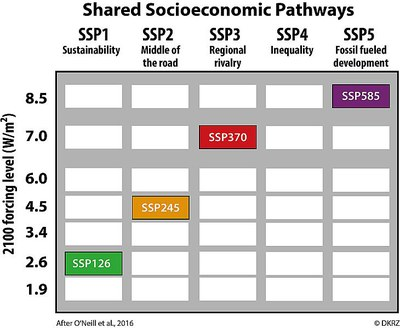
\includegraphics[width=0.5\textwidth]{figures/ssp_rcp_matrix.jpeg}
  \end{center}
  \caption[Overview CMIP6 SSP RCP Scenarios]{Combinations of \acp{ssp} and \acp{rcp} leading to scenarios comparable to the old \acp{rcp}. The vertical axis describes the old \ac{rcp} variant of a forcing level in 2100, while the horizontal axis are the \acp{ssp} 1 to 5. In combination, they define the new scenarios. \cite{bottinger_michael_ssp_nodate}}
  \label{fig:ssprcp}
\end{figure}


\section{Dataset description}




\subsection{Resolutions and Dimensions}
\label{sec:dataset-description}

In terms of spatial resolution, \ac{mpige6} comes in three variants: The low resolution variant MPI-ESM1.2-LR with a horizontal resolution of roughly $1.8^\circ$ longitude/latitude resolution in the atmospheric part and $0.4^\circ$ lon/lat for the ocean, the high resolution variant MPI-ESM1.2-HR with a horizontal resolution of $1.0^\circ$/$0.4^\circ$ for atmosphere/ocean and the extreme high resolution MPI-ESM1.2-XR with $0.5^\circ$/$0.4^\circ$ for atmosphere/ocean. 
Each variant has a vertical resolution of 47 levels for the atmosphere and 40 levels for the ocean.
With increasing spatial resolution comes decreased availability of other variables such as simulation members, covered time period, and implemented scenarios. 
Although \cite{olonscheck_new_2023} reports 30 members for each simulation (for the LR variant), in the actual dataset available for this work, 50 members were simulated. 

In terms of time resolution, \ac{mpige6} provides very few, limited variables in 3 hour intervals and most variables in a 6 hour interval.  
A complete list of the variables can be seen in \cite[Table 3]{olonscheck_new_2023}, the variables necessary for this thesis are listed in Table~\ref{tab:thesisVariables}. 

\begin{table}[bht]
\centering
\caption{Variables necessary for this thesis, derived from \cite{olonscheck_new_2023}}
\begin{tabular}{l|l|l|l}
  \label{tab:thesisVariables}
\textbf{Name} & \textbf{Parameter Long Name} & \textbf{Unit}                & \multicolumn{1}{l}{\textbf{Vertical Levels}}  \\ 
\hline
\textit{hus}              & Specific Humidity            & $1$                        & 47                                            \\
\textit{ua}               & Eastward (Zonal) Wind        & $ms^{-1}$              & 47                                            \\
\textit{va}               & Westward (Meridional) Wind   & $ms^{-1}$              & 47                                            \\
\textit{ps}               & Surface Air Pressure         & $Pa$                           & 1                                             \\
\textit{pr}               & Precipitation                & $kg~m^{-2} s^{-1}$ & 1    \\                                        
\textit{psl}               & Sea Level Pressure                & $Pa$ & 1            \\                                
\end{tabular}
\end{table}


\subsection{Vertical Hybrid Sigma Pressure Layers}
\label{sec:hybridsigma}

Regarding vertical levels, all variables were not available in fixed pressure layers but in the so-called \textit{ hybrid sigma pressure coordinates}. 
In comparison to fixed pressure layers (such as $1000 ~hPa$, $750 ~hPa$\dots), hybrid sigma pressure coordinates follow the terrain (mountains, valleys, etc.). 
Essentially, sigma vertical levels are given as fractions of the surface pressure $P_S$ at any point, following the equations in \cite{eckermann_hybrid_2009}: 

\begin{equation}
\label{eq:sigma-definition}
\sigma = h(p,P_S) = \frac{p - P_{top}}{P_S - P_{top}}
\end{equation}

Here, $p \in [P_S, P_{top}]$ is a pressure level. 
It was proposed that instead of providing pressure levels at pure fractional levels, it would be better to smoothly converge from terrain following fractions (sigma levels) at lower (i.e., near the earth surface) levels to isobaric (i.e., same pressure) levels in higher altitudes. 
This approach has both numerical and practical advantages.
There are also alternatives for $h(p, P_S)$, but a final form\footnote{The equations that lead to that can be seen in \cite{eckermann_hybrid_2009}} is used to calculate pressure levels at any discrete sigma level $\tilde{\eta}$:

\begin{equation}
\label{eq:hybrid-sigma}
p(\tilde{\eta}, P_S) = A(\tilde{\eta}) + B(\tilde{\eta}) (P_S - P_{top})
\end{equation}


$A(\tilde{\eta})$ is a vertical shift, which is close to zero at low levels, and $B(\tilde{\eta})$ is a fraction of the pressure range $(P_S - P_{top})$, which is close to zero at high levels. 

\begin{figure}
  \begin{center}
    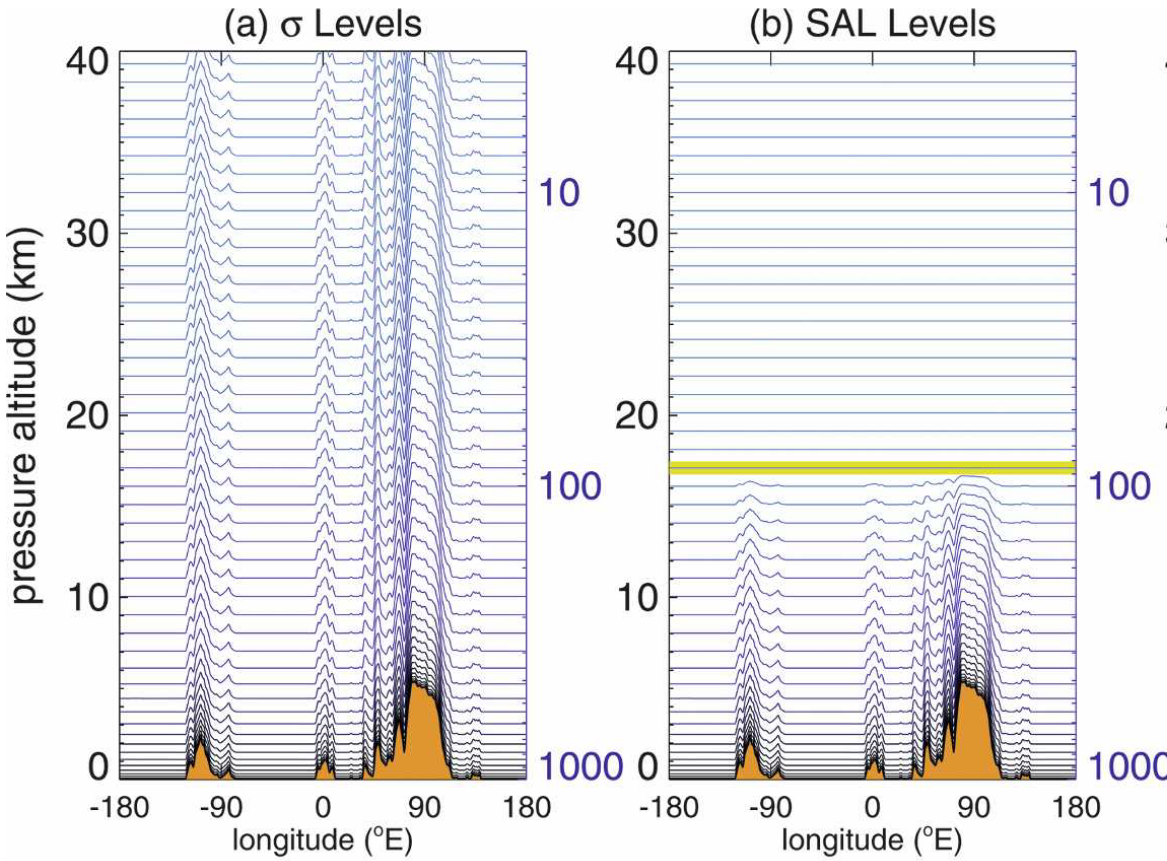
\includegraphics[width=0.65\textwidth]{figures/hybrid_sigma_pressure_layers.png}
  \end{center}
  \caption[Illustration of Hybrid Sigma Pressure Layers]{Examples of (hybrid) sigma pressure layers. a) shows sigma layers like in Equation \ref{eq:sigma-definition}, while b) shows a hybrid approach in the form of Equation \ref{eq:hybrid-sigma} \cite{eckermann_hybrid_2009}}\label{fig:hybrid-sigma}
\end{figure}



Using Equation~\ref{eq:hybrid-sigma} results in levels of equal pressure thickness, which merge to isobaric layers at higher altitudes. 
\citeauthorwork{olonscheck_new_2023} does not report their exact approach to $A(\tilde{\eta})$ and $B(\tilde{\eta})$ in \ac{mpige6}, but every data set that uses hybrid sigma pressure levels contains variables $ap(lev)$, $b(lev)$ and the pressure level field $ps(lon, lat, time)$, from which the pressure at any point and level can be calculated with:

\begin{equation}
\label{eq:mpige-sigma-hybrid-pressure}
p(lev, lon, lat, time) = ap(lev) + b(lev) ps(lon, lat, time)
\end{equation}


The upper pressure limit can be ignored in Equation~\ref{eq:mpige-sigma-hybrid-pressure} since the upper border is zero in \ac{mpige6}.


\subsection{Structure of the data}

The data is available in the high performance computing cluster of the DKRZ\footnote{Deutsches Klimarechenzentrum (en.: German Center for Climate Calculation)}, the structure can be seen in Figure \ref{fig:data-structure}.

\begin{figure}[htb]
  \begin{center}
    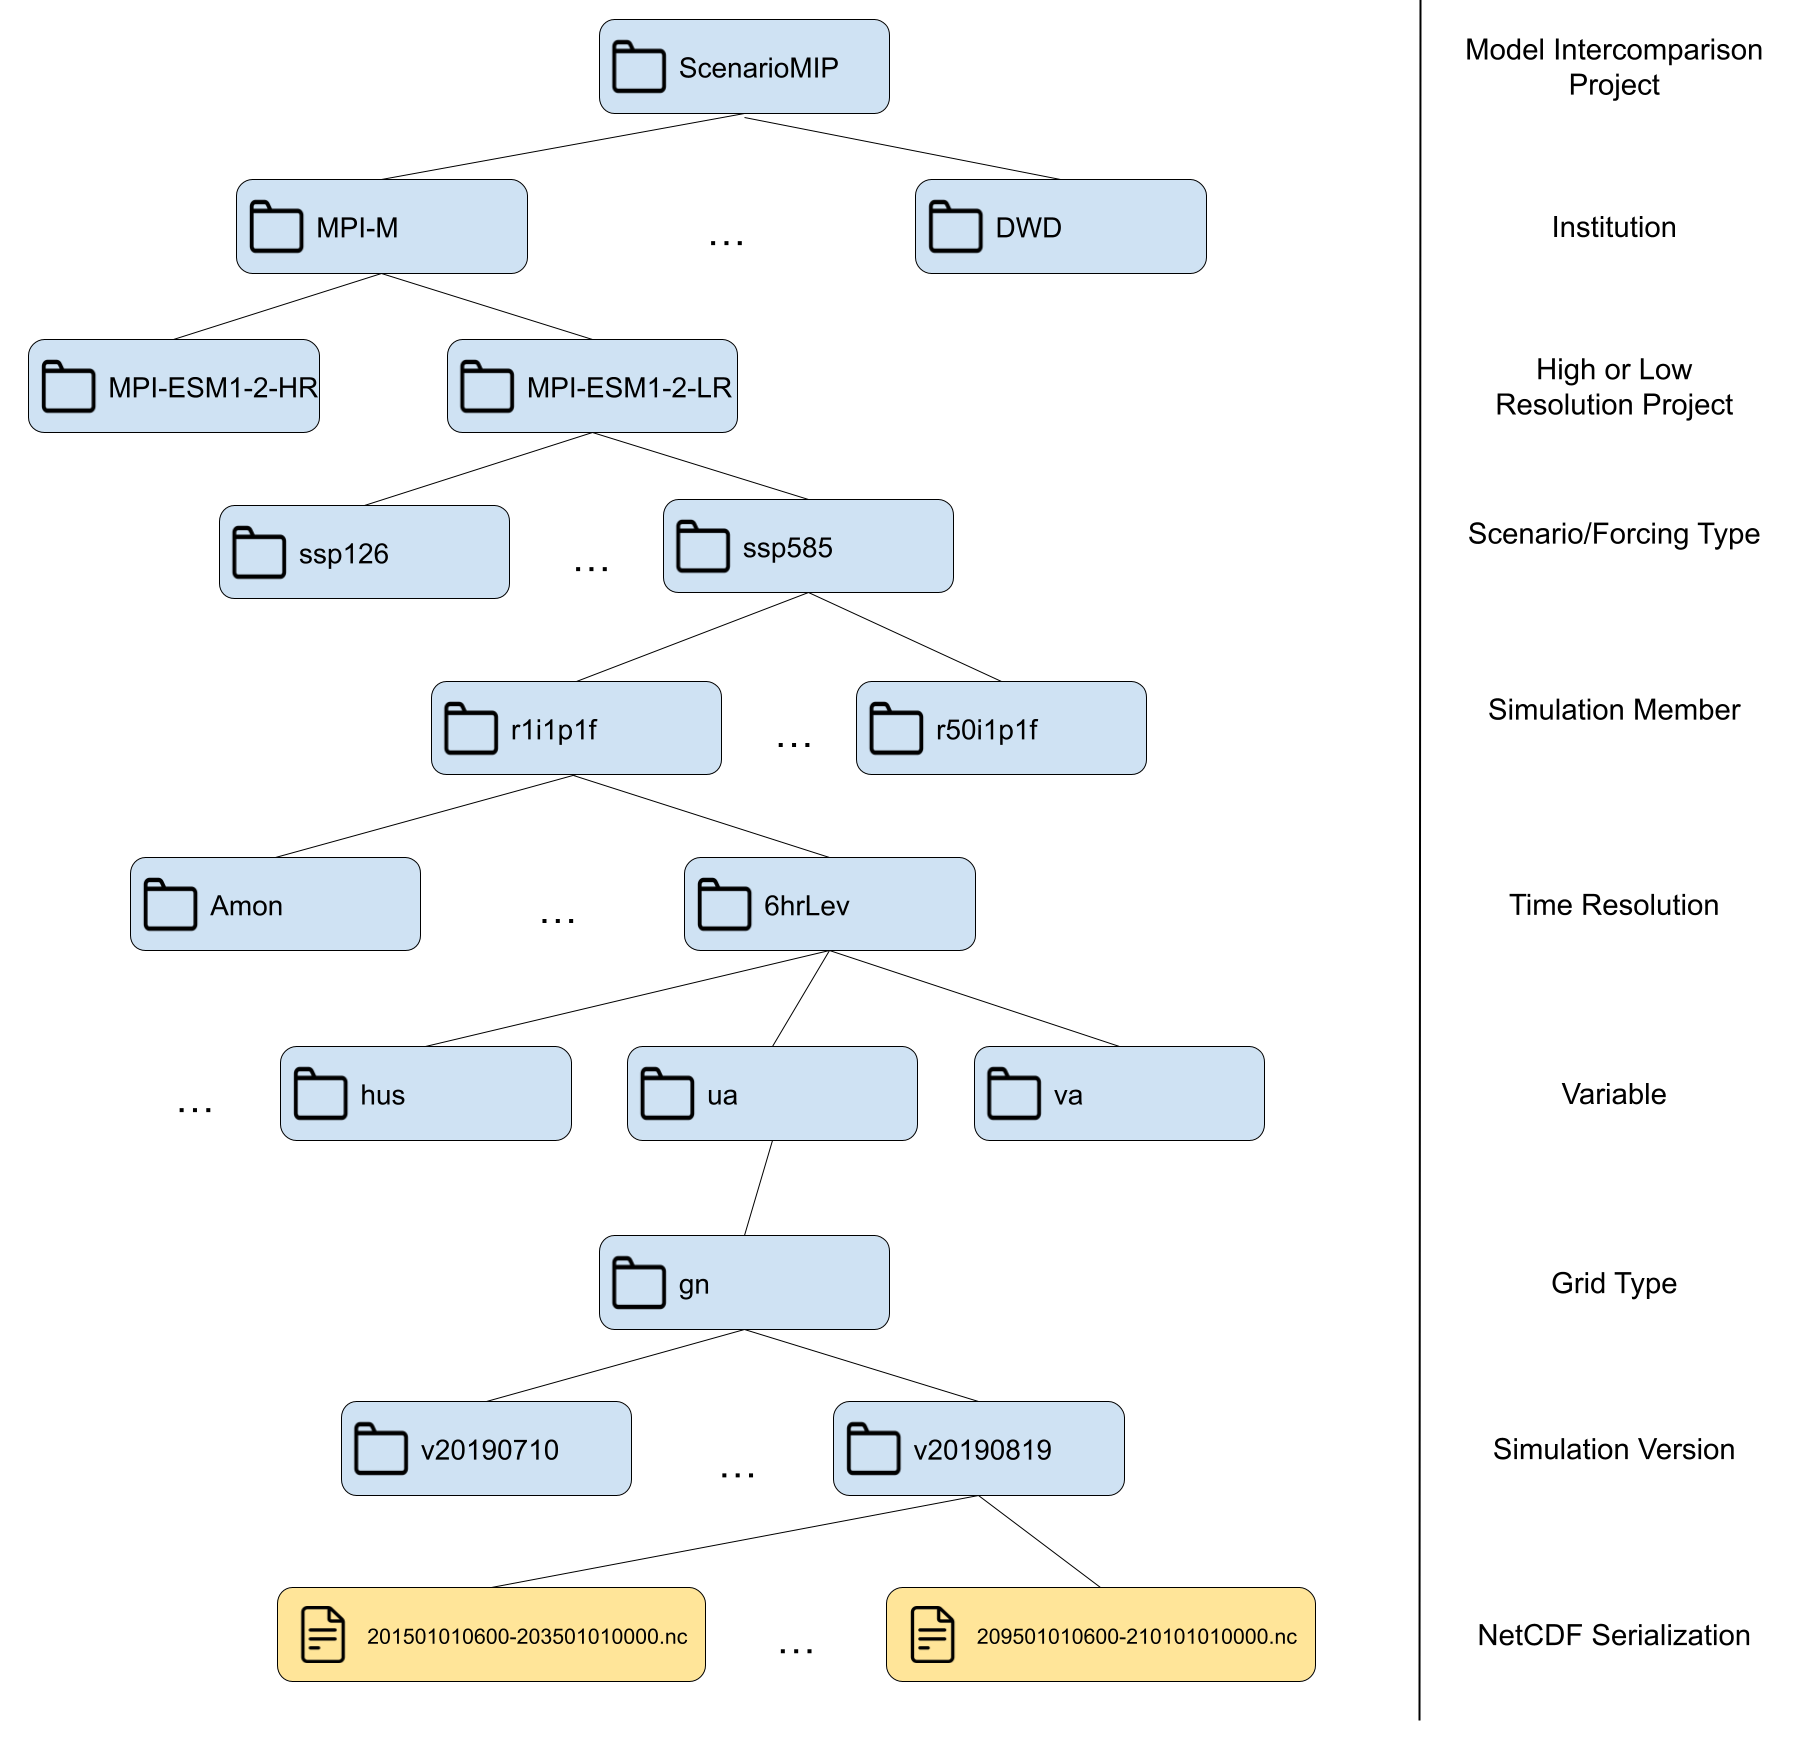
\includegraphics[width=0.75\textwidth]{figures/data_structure.png}
  \end{center}
  \caption[Illustration of Data Structure MPI GE CMIP6]{Structure the data is available on the DKRZ cluster. Example is given for ScenarioMIP, but applies as well for historical and piControl.}\label{fig:data-structure}
\end{figure}

The root folder is a \ac{mip}, for example, ScenarioMIP or the \ac{cmip} core, followed by the institution and resolution category (see Section~\ref{sec:dataset-description}). 
After a hierarchy of forcing types (e.g., \ac{ssp}, historical, piControl), member IDs and time resolutions, the variable (e.g., \textit{hus} for specific humidity) can be selected. 
After the grid type (only \textit{gn} is available) the version directory contains the actual data, serialized in the NetCDF4 format (which is based on HDF5 \cite{folk_overview_2011}) and divided into time scopes of up to 20 years. 
The version is named after the date of the simulation and, since a later version indicates a fix in the older version, it is generally advisable to choose the latest version for each variable.


\subsection{NetCDF Datasets}

The goal of the Network Common Data Format (NetCDF) was to create a machine-independent format for representing scientific data. 
It consists of an abstraction for storing multidimensional data, an implementation of said abstraction with a data format, and a library supporting that data format. 
It is modeled for supporting scientific datasets consisting of multiple, named, multidimensional variables together with their reference grid/coordinate system and some metadata properties.
Every variable consists of a type (e.g., scalars, byte arrays, characters, floating-point numbers), a shape defined by a vector of dimensions, and auxiliary properties as key-value pairs (e.g., physical unit, other names, important notes). \cite{rew_netcdf_1990}

\begin{figure}[htb]
  \begin{center}
    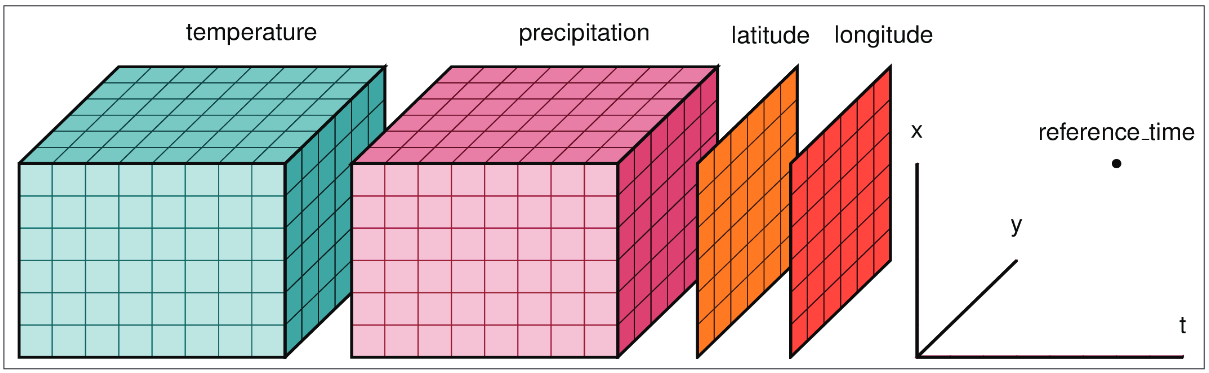
\includegraphics[width=0.95\textwidth]{figures/netcdf_visual_example.png}
  \end{center}
  \caption[Multidimensional Dataset Illustration]{An example of a named multidimensional dataset from \cite{hoyer_xarray_2017}: Precipitation and temperature are the variables while x, y and t are dimensions. Longitude and latitude are coordinates (also variables) defined by x and y.}
  \label{fig:example_dataset_structure}
\end{figure}

Figure~\ref{fig:example_dataset_structure} shows an example of the said structure in the form of a meteorological dataset: $x$, $y$, and $t$ are the dimensions, named integers representing the shape of variables. 
Precipitation and temperature are three-dimensional variables, while longitude and latitude are coordinates of the grid, giving a reference for the location of the grid. The dimensions of the dataset are x, y and t, giving both variables the shape $(x, y, t)$. \cite{hoyer_xarray_2017}
